\documentclass[11pt]{article}

\usepackage[margin=1in]{geometry}
\usepackage[english]{babel}
\usepackage[utf8]{inputenc}
\usepackage[T1]{fontenc}
\usepackage{lmodern}
\usepackage{microtype}
\usepackage{amsmath, amssymb}
\usepackage{graphicx}
\usepackage{booktabs}
\usepackage{hyperref}
\usepackage[backend=biber, style=numeric, sorting=none]{biblatex}
\addbibresource{refs.bib}

\hypersetup{
  colorlinks=true,
  linkcolor=black,
  citecolor=black,
  urlcolor=blue
}

\title{Triangulating Migraine Genetics, Autonomic Dysregulation, and CGRP Signaling: A Computational Synthesis Motivated by POTS--Migraine Comorbidity}
\author{Julian Quick}
\date{\today}

\begin{document}
\maketitle

\begin{abstract}
Migraine and Postural Orthostatic Tachycardia Syndrome (POTS) co-occur clinically far above population baselines, yet the field has no shared mechanistic model. Migraine genetics is mature (123 GWAS loci) and Calcitonin Gene-Related Peptide (CGRP)--targeting therapies are clinically effective; POTS genetics is essentially absent due to data scarcity, forcing any computational investigation of the comorbidity to triangulate rather than cross-reference. We do that in two phases. \emph{Phase~2 (pre-registered)} executes three tests on the Hautakangas et al.\ (2022) migraine GWAS gene set: PPI network proximity in BioGRID$\cup$IntAct ($22{,}091$ nodes, $1{,}109{,}901$ edges) to the CGRP-selective receptor anchor (CALCRL+RAMP1) with a degree-matched null and four control diseases; focused autonomic over-representation against a length-quintile-matched permutation null; and GTEx v8 tissue expression. The proximity observation $z = +3.54$ ($p = 0.004$) does not pass the pre-registered specificity criterion (three of four control diseases show the same direction at similar magnitude); set-level autonomic over-representation is null ($k = 2$ vs $\mathbb{E}[k] = 1.9$, $p = 0.57$); GTEx expression of migraine and CGRP anchors is concentrated in autonomic-relevant tissues (median log$_2$(TPM+1) $\sim$3.4--3.8 in tibial artery / aorta / coronary artery vs 0.8 in whole blood). \emph{Phase~3 (post-hoc, explicitly motivated by the Phase~2 synthesis)} adds two paper-internal probes of literature-level observations: an ESR1 ChIP-seq promoter-occupancy enrichment using ReMap2022 non-redundant peaks (866{,}869 peaks merged across 448 datasets and 24 biotypes, sensitivity sweep over peak-stringency thresholds), and an OpenTargets Genetics locus-to-gene sensitivity layer. The ESR1 ChIP-seq test is null at every stringency: CGRP-pathway, migraine-GWAS, and autonomic gene sets all show ESR1 promoter occupancy at or below length-matched background. This rules out direct ER binding to CGRP-pathway promoters as a general property of the ER-responsive cell types that dominate ChIP-seq depositions (MCF-7, T47D, ZR-75-1, Ishikawa, breast / endometrial tissue), and refines the estrogen-bridge hypothesis toward indirect / distal mechanisms---most naturally regulation of CGRP \emph{release} rather than transcription, which is what Krause et al.\ (2021) actually demonstrated mechanistically. The OpenTargets L2G layer is informative: CALCA's genetic-association score (0.753) sits in the range of canonical migraine GWAS hits (PRDM16 0.798, TRPM8 0.816, FHL5 0.855), CALCB's is moderate (0.450, a graded rather than binary asymmetry), and CALCRL/RAMP1/CRCP have no \texttt{genetic\_association} datatype recorded at all in the OpenTargets evidence ledger---their non-zero overall scores derive entirely from drug-target and literature channels. The synthesis consolidates three contributions, each at a different epistemic level. (1)~The CGRP \emph{ligand--receptor asymmetry} originally reported by Hautakangas et al.\ (2022) is now reproducible across five analytical lenses: the 2022 GWAS, 2025 fine-mapping, eQTL-integrated TWAS, our PPI proximity test, and OpenTargets L2G aggregated genetic-association scores. The lenses are not statistically independent (they share much of the underlying GWAS data) but they apply different inferential machinery, and the asymmetry is consistent across all five. (2)~The migraine and CGRP gene sets share a robust tissue distribution peaking in nerve and arterial tissues, and the cross-species harmonized cell atlas of trigeminal and dorsal-root ganglia~\cite{bhuiyan_2024_drg_tg_atlas} explicitly defines a \textit{Calca}$^+$\textit{Adra2a} neuronal subtype, which operationalizes the CGRP--autonomic convergence at single-cell resolution. (3)~The estrogen$\rightarrow$CGRP convergence at the organismal level (POTS genomics, estrogen-mediated CGRP-release modulation, $\sim$80--90\% female predominance shared by both diseases) is real, but is \emph{not} mediated by direct ER binding to CGRP-pathway promoters. Direct cross-trait analysis of the migraine--POTS comorbidity remains bottlenecked on a properly powered POTS GWAS cohort that does not yet exist; this synthesis identifies the data-collection priority and the specific analyses that become tractable once it does.
\end{abstract}

\section{Introduction}
\label{sec:intro}

\paragraph{Clinical motivation.} Migraine is a common, disabling neurological disorder with a lifetime prevalence near 15\% and substantial sex bias toward women. A meaningful subpopulation of migraine patients also meets criteria for Postural Orthostatic Tachycardia Syndrome (POTS) or related autonomic disorders, and the clinical overlap is well recognized in dysautonomia and headache clinics. The mechanistic relationship, however, is not settled: migraine attacks and POTS episodes share triggers (postural change, sleep loss, dehydration, hormonal shifts), share symptom domains (headache, brain fog, sensory sensitivity), and plausibly share signaling substrates (sympathetic activation, vascular instability, sensory nerve sensitization), but the literature has not unified them under a single computational framework.

\paragraph{Mechanistic anchor: CGRP.} The dominant validated migraine target at the molecular level is Calcitonin Gene-Related Peptide (CGRP). Anti-CGRP monoclonal antibodies and small-molecule receptor antagonists (gepants) are FDA-approved migraine therapies, providing strong perturbational evidence that CGRP signaling participates causally in migraine attacks. CGRP is not a migraine-specific molecule: it is a sensory-nerve neuropeptide with roles in vascular regulation, neurogenic inflammation, and protective stress responses. These roles are autonomic-adjacent.

\paragraph{The data asymmetry.} Migraine GWAS is mature, with the largest meta-analyses involving hundreds of thousands of cases. POTS GWAS is essentially absent: the disorder is under-coded in biobanks, often misdiagnosed, and lacks a large genetic cohort. This asymmetry rules out a direct migraine-vs-POTS genetic cross-reference and forces a triangulation strategy: use migraine genetics as the signal-rich anchor, build mechanism-driven gene sets that proxy POTS-relevant biology (autonomic, adrenergic, sympathetic), and ask whether migraine genetic risk converges on those proxies and on CGRP signaling more than chance would predict.

\paragraph{The question this paper addresses.} \emph{Does migraine genetic risk, when intersected with curated autonomic and CGRP gene sets and analyzed through protein--protein interaction network proximity, sit closer to autonomic biology than degree-matched random gene sets, and what does that imply for the POTS--migraine--CGRP axis?}

\paragraph{Honest scoping.} This work is a computational synthesis and secondary analysis. It does not generate new wet-lab data, does not establish causation, and cannot resolve POTS genetics in the absence of POTS cohorts. Its ceiling claim is \emph{consistency with} an autonomic dysregulation hypothesis. A clean negative result---migraine genetics does not preferentially overlap autonomic biology more than matched neurological conditions---would itself be informative.

\paragraph{Contributions.} The contributions live at distinct epistemic levels, and we name them explicitly to avoid conflating literature-level synthesis with paper-internal data.
\begin{itemize}
  \item Frame the POTS--migraine--CGRP triangulation as a tractable computational object given the current data asymmetry, and provide a comprehensive literature review and explicit gap analysis establishing the proposed work as partially-novel.
  \item \emph{Phase 2: pre-registered tests.} Execute three analyses on Hautakangas et al.\ (2022) migraine GWAS--prioritized genes against published data: PPI network proximity to the CGRP-selective receptor anchor with a degree-matched null and four specificity controls, focused autonomic over-representation against a length-matched permutation null, and GTEx tissue expression across pre-registered autonomic-relevant tissues.
  \item \emph{Phase 3: post-hoc tests motivated by the Phase 2 synthesis.} Two paper-internal analyses of literature-level observations: (a)~an ESR1 ChIP-seq promoter-occupancy enrichment test using ReMap2022 non-redundant peaks~\cite{hammal_2022_remap}, sensitivity-swept across peak-stringency thresholds, that empirically falsifies a ``direct ER $\rightarrow$ CGRP-promoter'' model of the estrogen bridge; (b)~an OpenTargets Genetics locus-to-gene sensitivity layer~\cite{ochoa_2023_opentargets} that confirms the CGRP ligand--receptor asymmetry through an independent, multi-source genetic-evidence aggregator. We label these as post-hoc to the locked Phase 2 pre-registration; both are falsification-oriented (they could have produced positives) and the protocols and seeds are fixed before running.
  \item Document that the CGRP \emph{ligand--receptor asymmetry} originally reported by Hautakangas et al.\ (2022) is reproducible across five analytical lenses: the 2022 GWAS, the 2025 fine-mapping, an eQTL-integrated TWAS~\cite{ghaffar_2023_migraine_eqtl_twas}, the PPI network-proximity test reported here, and OpenTargets L2G aggregated genetic-association scores. These lenses share much of the underlying GWAS data and are not statistically independent, but they apply different inferential machinery (variant-level association, statistical fine-mapping, TWAS imputation, network distance, multi-source evidence aggregation) and yield consistent answers. The asymmetry is graded rather than binary---CALCB carries moderate L2G genetic-association evidence ($0.450$) while CALCRL/RAMP1/CRCP carry none---but it is no longer a single-paper observation, and any future causal model of CGRP-pathway involvement in migraine genetics must accommodate it.
  \item Articulate the estrogen$\rightarrow$CGRP convergence as a level-stratified hypothesis. \emph{At the organismal level} the convergence is real: the first systematic POTS genomic study~\cite{qu_2025_pots_genetics} recovers HALLMARK\_ESTROGEN\_RESPONSE\_EARLY, estrogen withdrawal modulates trigeminovascular CGRP release~\cite{krause_2021_estrogen}, and both diseases share $\sim$80--90\% female predominance. \emph{At the molecular promoter-binding level}, the Phase 3 ESR1 ChIP-seq test returns null at every stringency: ER does not preferentially bind CGRP-pathway promoters at the proteome-wide tendency dominated by ER-responsive cell lines, ruling out the simplest direct-transcription mechanism for that class of cells. The bridge must therefore be indirect---release modulation, distal enhancer regulation, or intermediate signaling through autonomic substrates such as the \textit{Calca}$^+$\textit{Adra2a} trigeminal subtype reported by Bhuiyan et al.\ (2024)~\cite{bhuiyan_2024_drg_tg_atlas}.
  \item Identify the bottleneck. The pre-registered triangulation we executed delivers two negatives, one directional finding, and a falsified molecular sub-hypothesis precisely because the relevant tests are weakest where the data are weakest---around the receptor side of the CGRP pathway and around POTS genetics generally. Several of the questions this paper cannot answer (cross-trait LDSC of migraine and POTS, sex-stratified shared-loci tests, direct estrogen$\rightarrow$CGRP$\rightarrow$autonomic causal inference) become directly tractable once a properly powered POTS cohort exists. The most useful contribution to the broader research agenda may therefore be making the data-collection priority explicit.
\end{itemize}

\section{Background}
\label{sec:background}

\subsection{Migraine genetics}
\label{sec:bg-migraine}

Migraine common-variant genetics is mature. Successive meta-analyses traced an arc from twelve loci across roughly twenty-three thousand cases~\cite{anttila_2013_migraine_gwas}, to thirty-eight loci across sixty thousand~\cite{gormley_2016_migraine_gwas}, to one hundred and twenty-three loci in the Hautakangas et al.\ 2022 meta-analysis of 102{,}084 cases and 771{,}257 controls~\cite{hautakangas_2022_migraine_gwas}, with multiethnic confirmation across European, East Asian, African American, and Hispanic/Latino cohorts identifying a further set of sex-specific loci~\cite{choquet_2021_multiethnic}. A 2025 fine-mapping reanalysis of approximately ninety-eight thousand cases yielded one hundred and eighty-one credible variant sets, with seven variants reaching posterior inclusion probability greater than 0.9~\cite{hautakangas_2025_migraine_finemapping}. Trans-ancestry coverage is expanding, though smaller non-European cohorts remain underpowered relative to the European mega-analyses~\cite{liu_2024_han_chinese_migraine_gwas}.

Twin-study heritability estimates concentrate at $\approx$0.36--0.48 across more than fifty studies~\cite{olofsson_2024_migraine_twin_review}, indicating that a substantial fraction of liability is genetic but that common-variant GWAS still leaves heritability unaccounted for, motivating pathway-level integration. The rare-variant frontier is now opening: a deCODE-led analysis across $\approx$1.3 million individuals identified large-effect rare variants in \textit{PRRT2} (migraine with aura, OR $\approx$ 5.4), \textit{SCN11A} (protective), and a cis-regulatory variant in \textit{KCNK5}~\cite{bjornsdottir_2023_rare_migraine_variants}, while UK Biobank exome-wide analyses extend the monogenic familial hemiplegic migraine genes (\textit{CACNA1A}, \textit{ATP1A2}, \textit{SCN1A}; reviewed in~\cite{alfayyadh_2024_hemiplegic_migraine_review}) into population-level sub-Mendelian risk~\cite{staehr_2025_fhm_ukb_exome}. A 2024 narrative review frames the integrated picture as convergence on excitatory--inhibitory imbalance and neurovascular pathways~\cite{sutherland_2024_migraine_genetics_review}.

Two facts from this literature are load-bearing for our triangulation. First, Hautakangas et al.\ identified a chromosome 11 locus containing \textit{CALCA}/\textit{CALCB} (the genes encoding the CGRP and adrenomedullin ligands) as genome-wide significant, but the paper explicitly notes that ``none of the genes encoding CGRP receptor proteins (\textit{CALCRL}, \textit{RAMP1} or \textit{RCP}) show a statistically comparable association (all $P > 10^{-4}$)''~\cite{hautakangas_2022_migraine_gwas}. The 2025 fine-mapping does not nominate the receptor-complex genes as causal either~\cite{hautakangas_2025_migraine_finemapping}, and a transcriptome-wide association study integrating eQTLs across forty-nine GTEx tissues~\cite{ghaffar_2023_migraine_eqtl_twas} also fails to surface them. The ligand--receptor asymmetry is therefore not an artifact of statistical thresholding in any single study; it is reproducible. Second, no major migraine GWAS to date has run pathway enrichment specifically on autonomic, sympathetic, parasympathetic, or adrenergic gene sets. Hautakangas et al.\ used MAGMA against MSigDB-curated and GO collections; Gormley et al.\ reported broad vascular and smooth-muscle tissue enrichment; Choquet et al.\ surfaced flavonoid glucuronide and ascorbate--aldarate metabolism via FUMA; the 2024 Sutherland review does not catalogue any autonomic-specific analysis. The autonomic dimension is therefore an open question, and the focus of this synthesis.

\subsection{CGRP biology and migraine pharmacology}
\label{sec:bg-cgrp}

The molecular case for CGRP signaling in migraine rests on three converging lines of evidence: a defined biosynthetic and receptor architecture, perturbational evidence that exogenous CGRP provokes migraine-like attacks, and pharmacological evidence that blocking CGRP signaling at either ligand or receptor prevents and aborts them.

\paragraph{Architecture.} CGRP arises from \textit{CALCA} via tissue-specific alternative RNA processing: a calcitonin-encoding mRNA predominates in thyroid C cells, while a CGRP-encoding mRNA predominates in neurons~\cite{amara_1982_calca}. The active receptor is a heterodimer of the calcitonin-receptor-like receptor (CLR / \textit{CALCRL}) and receptor-activity-modifying protein 1 (RAMP1), with receptor component protein (RCP / \textit{CRCP}) supporting Gs coupling. The 3.3-\AA\ cryo-EM structure of the active human CGRP receptor in complex with peptide and Gs heterotrimer~\cite{liang_2018_cgrpr_cryoem} shows that RAMP1 sits at the CLR transmembrane TM3/4/5 interface and stabilizes ECL2, contacting CGRP only minimally, consistent with allosteric modulation of CLR rather than direct ligand binding.

\paragraph{Perturbational evidence.} Intravenous infusion of human $\alpha$-CGRP at 2~\textmu g/min for twenty minutes provoked headache in all twelve migraineurs without aura tested in a double-blind crossover, versus one in twelve under placebo, with three patients meeting full IHS migraine-without-aura criteria~\cite{lassen_2002_cgrp_provocation}. This established that exogenous CGRP is sufficient to provoke migraine-like attacks in susceptible individuals.

\paragraph{Pharmacological evidence.} Four monoclonal antibodies targeting either the CGRP ligand (fremanezumab~\cite{silberstein_2017_halo_fremanezumab}, galcanezumab~\cite{stauffer_2018_evolve1_galcanezumab}, eptinezumab~\cite{lipton_2020_promise2_eptinezumab}) or the CGRP receptor (erenumab~\cite{goadsby_2017_strive_erenumab}) have demonstrated approximately 3.5--4.7 monthly migraine-day reductions in episodic migraine and 4.3--4.6 in chronic migraine across pivotal phase 3 trials, with $\geq$50\% responder rates near 40--60\% versus 18--27\% on placebo. Three orally administered small-molecule receptor antagonists (gepants) reproduce this signal: rimegepant and ubrogepant for acute treatment, with two-hour pain freedom roughly twice placebo~\cite{croop_2019_rimegepant,dodick_2019_achieve1_ubrogepant}, and atogepant for daily prevention with monthly migraine-day reductions of 3.7--4.2 versus 2.5 on placebo~\cite{ailani_2021_advance_atogepant}. A modern review consolidates these findings into the trigeminovascular framework and locates the primary site of action at the trigeminal ganglion, peripheral and outside the blood--brain barrier~\cite{edvinsson_2018_cgrp_review}.

\paragraph{CGRP outside migraine, and the autonomic relevance.} CGRP is not solely a pain neuropeptide. A comprehensive physiological review documents CGRP as among the most potent endogenous vasodilators known, a mediator of neurogenic inflammation alongside substance P, and a tonic counter-regulator of the renin--angiotensin--aldosterone and sympathetic systems in cardiovascular regulation~\cite{russell_2014_cgrp_physiology}. Sensory afferents---including perivascular trigeminal afferents---are the primary source of circulating CGRP under physiological conditions. Postmarketing pharmacovigilance corroborates the autonomic relevance: a 2021 case series identified sixty-one reports of substantial blood-pressure elevation on erenumab, with median systolic increase of 39~mmHg, leading to a 2020 US label update adding hypertension to Warnings and Precautions~\cite{saely_2021_erenumab_hypertension}. If pharmacological blockade of CGRP receptor signaling raises blood pressure, then endogenous CGRP performs autonomic work at baseline, not only nociceptive work during attacks. This is the molecular substrate that connects migraine pharmacology to the autonomic phenotypes addressed in the next subsection.

\subsection{Autonomic dysfunction and POTS}
\label{sec:bg-pots}

\paragraph{Definition and subtypes.} The 2015 Heart Rhythm Society consensus statement defines POTS as a sustained heart-rate increase of at least 30~bpm (40~bpm in adolescents) within ten minutes of standing, in the absence of orthostatic hypotension, accompanied by chronic symptoms of orthostatic intolerance for at least three months~\cite{sheldon_2015_hrs}. Three operational subtypes are distinguished---neuropathic (patchy peripheral sympathetic denervation, especially lower limb), hyperadrenergic (upright plasma norepinephrine $>$600~pg/mL with rising blood pressure), and hypovolemic (reduced red-cell mass and plasma volume)---though the subtypes overlap in most patients~\cite{raj_2013_pots}. The 2021 NIH Expert Consensus reaffirms POTS as a heterogeneous syndrome with overlapping mechanisms and no single unified pathophysiology, documents the strong female predominance (approximately 80--94\%), and identifies migraine, Ehlers--Danlos syndrome, mast-cell activation syndrome, and ME/CFS as the principal comorbidities~\cite{vernino_2021_nih}.

\paragraph{POTS--migraine comorbidity.} The clinical overlap is robust but quantitatively unstable. A 2022 systematic review and meta-analysis found a pooled prevalence of migraine in POTS of 36.8\%, with a 95\% confidence interval of 2.9--70.7\% across twenty-three studies and substantial between-study heterogeneity~\cite{ray_2022_metaanalysis}. Larger clinic-based cohorts report higher rates: in a 2023 hEDS cohort, migraine prevalence was 67\% and POTS prevalence was 61\%, with a mean of 10.45 co-diagnoses per individual~\cite{halverson_2023_heds}, and an earlier controlled study found 75\% migraine prevalence in women with joint hypermobility syndrome versus 43\% in controls~\cite{bendik_2011_hypermobility}. The strongest existing narrative review of POTS--migraine comorbidity identifies the most plausible mechanistic overlaps as sympathetic-nervous-system dysregulation, central and peripheral hemodynamic alterations, and central sensitization---but conspicuously does not center CGRP as a bridging mechanism~\cite{mueller_2022_potsmigraine}. Independently of comorbid POTS, migraineurs themselves show measurable cardiac autonomic dysregulation: reduced heart-rate variability, lower SDNN and triangular index, with parasympathetic dysfunction predominating during the ictal phase and sympathetic abnormalities also present~\cite{zhang_2021_hrv}. An autonomic-migraine axis is therefore intrinsic to the migraine phenotype, not solely a feature of the POTS-comorbid subgroup.

\paragraph{POTS genetics.} POTS genetics was, until very recently, essentially absent. The signature monogenic example is heterozygous loss of function in the norepinephrine transporter (\textit{SLC6A2}, A457P, $>$98\% LoF) in a family with familial orthostatic intolerance, establishing impaired norepinephrine clearance as a molecular driver of hyperadrenergic orthostatic intolerance~\cite{shannon_2000_net}. Beyond this, only a single replicated candidate-gene signal exists: the \textit{GNB3} C825T polymorphism is overrepresented (TT genotype 45.8\% vs 20.0\%, $p=0.036$) in pediatric POTS~\cite{nakao_2012_gnb3}. The first systematic genomic interrogation of POTS appeared in 2025: a combined GWAS and whole-exome sequencing study in 207 European cases and 4{,}063 controls, with WES on 87 cases~\cite{qu_2025_pots_genetics}. No common variants reached genome-wide significance, but the authors performed an over-representation analysis on the 5{,}670 SNPs reaching nominal significance ($P < 0.05$), and rare-variant burden analysis separately identified fifty-five genome-wide-significant genes harboring ninety-two pathogenic or likely-pathogenic variants. The GWAS over-representation analysis recovered---among other gene sets---HALLMARK\_ESTROGEN\_RESPONSE\_EARLY ($P = 3.78 \times 10^{-4}$, FDR $= 0.019$); the authors note that estrogen-response genes ``could potentially play a role in POTS, given the higher prevalence of the condition in women.''

\paragraph{The estrogen bridge.} Estrogen is the most plausible endocrine substrate connecting the female sex bias of POTS, the female sex bias of migraine, and the CGRP system. A 2021 review establishes that estrogen withdrawal disinhibits trigeminovascular CGRP expression and release, and synthesizes the mechanistic axis by which ovarian steroids modulate CGRP-driven migraine pathophysiology~\cite{krause_2021_estrogen}. Combined with the rare-variant ``early estrogen response'' enrichment in POTS~\cite{qu_2025_pots_genetics}, the estrogen$\rightarrow$CGRP axis becomes the natural mechanistic bridge that the POTS--migraine literature has otherwise left unarticulated.

\subsection{Computational methods for cross-disease genetic synthesis}
\label{sec:bg-methods}

The proposed analyses draw on three method families: gene-level aggregation of GWAS summary statistics, pathway and tissue enrichment, and protein--protein interaction network proximity.

\paragraph{Gene-level aggregation.} MAGMA aggregates SNP-level $p$-values into gene-level statistics using a multiple-regression model that accounts for linkage disequilibrium, and supports competitive gene-set tests with covariate adjustment~\cite{deleeuw_2015_magma}. The FUMA platform wraps MAGMA together with positional, eQTL, and chromatin-interaction SNP-to-gene mapping, GTEx tissue enrichment, and MSigDB-based pathway tests in a versioned and reproducible pipeline~\cite{watanabe_2017_fuma}. GTEx v8 provides the eQTL substrate inside FUMA's SNP-to-gene mapping and supplies the tissue-enrichment statistics; coverage is 15{,}201 RNA-seq samples across 49 tissues in 838 donors~\cite{gtex_2020_atlas}.

\paragraph{Pathway enrichment.} Two complementary engines anchor the field. g:Profiler runs over-representation analysis against GO, KEGG, Reactome, WikiPathways, transcription-factor, miRNA, Human Protein Atlas, and Human Phenotype Ontology sources, with a hierarchical correction (g:SCS) tailored to redundant nested ontology terms~\cite{raudvere_2019_gprofiler}. Enrichr provides a Fisher-style server with combined-score ranking against more than 180 libraries spanning ontologies, pathways, drug perturbations, transcription factors, cell types, disease signatures, ARCHS4, DSigDB, and GTEx~\cite{kuleshov_2016_enrichr}. A long-standing methodological caveat applies to all such tests: competitive gene-sampling tests assume gene--gene independence, which is almost always violated, so subject-sampling (phenotype permutation) or LD-aware regression-based competitive tests are preferred over naive hypergeometric over-representation~\cite{goeman_2007_genesets}.

\paragraph{Network proximity.} Guney et al.\ define and benchmark several network-proximity measures (closest, shortest, kernel, centre, separation) between drug-target sets and disease-gene sets in the human interactome, with a degree-preserving randomization null that converts proximity into a $z$-score; ``closest'' distance with degree-binned random reference sets best discriminates effective from palliative drugs across 238 drugs and 78 diseases~\cite{guney_2016_proximity}. Menche et al.\ introduce the network-separation score $S_{AB}$ between two disease gene sets and derive the conditions under which a disease module is identifiable in an incomplete PPI network: overlapping modules ($S_{AB} < 0$) predict comorbidity, co-expression, and symptom similarity, while well-separated modules are clinically distinct~\cite{menche_2015_diseaseome}. The canonical degree-preserving null is the Maslov--Sneppen edge-rewiring procedure~\cite{maslov_2002_rewiring}, of which the Guney degree-binned random gene-set draw is a computationally cheaper equivalent.

\paragraph{PPI database choice.} Three resources dominate. STRING integrates physical and functional associations with per-edge confidence scores from text mining, experiments, databases, co-expression, and genomic context~\cite{szklarczyk_2023_string}; the inclusion of text-mining edges introduces a literature-bias hazard for any analysis involving heavily studied genes. BioGRID is an open, manually curated repository of physical, genetic, and chemical interactions with PubMed-anchored evidence codes~\cite{oughtred_2021_biogrid}, and IntAct is a PSI-MI-curated repository of binary interactions with detailed experimental annotation~\cite{deltoro_2022_intact}. For a hypothesis test asking whether migraine GWAS hits are closer to the CGRP receptor complex than chance, the literature-bias hazard of STRING is precisely the failure mode to avoid: \textit{CALCA}, \textit{CALCB}, \textit{RAMP1}, and \textit{CALCRL} are among the most heavily literature-studied genes in headache neuroscience, and text-mining edges would artificially shorten the distance between any well-studied gene set and the CGRP module. The methodologically conservative default is therefore the union of BioGRID and IntAct physical-only interactions, with STRING (high-confidence physical subnetwork, text-mining channel disabled) reported as a sensitivity analysis.

\section{Related Work and Gap Analysis}
\label{sec:related}

Each of the three legs of the proposed triangulation has been touched by published work, but no single computational object combines them, and the specific tests we plan have not been published.

\paragraph{Migraine GWAS pathway enrichment.} Generic enrichment using broad ontology and curated-pathway collections is fully covered by the source GWAS papers themselves. Hautakangas et al.\ used MAGMA against MSigDB-curated and GO collections~\cite{hautakangas_2022_migraine_gwas}; Choquet et al.\ used FUMA and DEPICT, surfacing flavonoid glucuronide biosynthesis and ascorbate--aldarate metabolism~\cite{choquet_2021_multiethnic}; Ghaffar and Nyholt used a transcriptome-wide association study integrating GTEx eQTLs across forty-nine tissues to prioritize vascular and inflammatory tissues~\cite{ghaffar_2023_migraine_eqtl_twas}. None of these analyses tested an autonomic, sympathetic, parasympathetic, or adrenergic-receptor gene set as a focused hypothesis with a permutation null distinct from the generic MSigDB and GO enrichments.

\paragraph{Migraine cardiovascular cross-trait genetics.} A 2020 LDSC analysis between migraine and forty-seven UK Biobank phenotypes plus external GWAS found genetic correlations $r_g = 0.10$ with diastolic blood pressure ($P = 5.4 \times 10^{-5}$) and $r_g = 0.063$ with systolic blood pressure, and additional correlations with heart disease and lipid panels~\cite{siewert_2020_crosstrait}. Notably, that forty-seven-trait panel does \emph{not} include heart-rate variability, orthostatic intolerance, syncope, or any POTS-related phenotype. A genome-wide cross-phenotype meta-analysis of migraine and blood pressure subsequently identified fourteen shared loci; \textit{ADRA2B}, encoding the alpha-2B adrenergic receptor, is the only adrenergic-receptor gene called out among shared loci, but the analysis did not perform a formal autonomic gene-set enrichment, did not run a network-proximity test against the CGRP receptor complex, and did not address POTS comorbidity~\cite{guo_2020_bp_migraine}. We are aware of no published LDSC genetic correlation between migraine and any autonomic or POTS-adjacent phenotype, and the only existing systematic POTS GWAS~\cite{qu_2025_pots_genetics} has not been cross-trait-analyzed with migraine.

\paragraph{Migraine drug-target and PPI work.} A 2024 druggable-genome Mendelian randomization study with colocalization on migraine GWAS surfaced twenty-one druggable migraine-associated genes; PPI was used as a downstream visualization, and \textit{CALCB}, \textit{CALCRL}, \textit{RAMP1}, and \textit{RAMP3} appear only as comparator known drug targets, not as a tested complex~\cite{zhang_2024_druggable}. A 2025 SMR/HEIDI--colocalization--PPI--enrichment pipeline on migraine GWAS prioritized eight genes interacting with known CGRP and 5-HT pathway drug targets and proposed forty-one repurposable drugs, but the construct is target prioritization rather than a permutation-null hypothesis test of proximity to a CGRP-receptor anchor~\cite{liu_2025_precision_target}. A migraine-subtype syncope GWAS tested only three pre-selected candidate variants (\textit{TRPM8}, \textit{GFRA1}, \textit{LRP1}), all non-significant~\cite{lin_2024_syncope_migraine}.

\paragraph{Closest conceptual cousin.} A 2024 arXiv preprint proposes a sympathetic-nervous-system theory of migraine linking sympathetic saturation, baroreceptor hyperexcitability, and downstream CGRP release, citing candidate genes (\textit{TRPM8}, \textit{PRDM16}, \textit{ATP1A2}) from prior literature~\cite{rappoport_2024_sns_migraine}. The framework is verbal and mechanistic; it performs no GWAS overlap, no gene-set enrichment, and no PPI network analysis. We cite it as motivating prior art for the autonomic--CGRP linkage, while noting that the computational test of that linkage has not been performed.

\paragraph{Verdict.} The state of the literature is therefore \emph{partially novel, leaning strongly novel} for the proposed work. (i) No published migraine GWAS pathway-enrichment analysis has tested autonomic or adrenergic gene sets as a focused hypothesis with a permutation null. (ii) No published LDSC has computed genetic correlation between migraine and a POTS-adjacent or HRV phenotype; existing cross-trait analyses stop at blood pressure. (iii) Published migraine PPI / network-pharmacology work has been target-prioritization, not CGRP-anchored proximity hypothesis testing with a degree-preserving null. (iv) The POTS-comorbidity-motivated framing is unaddressed in the published computational literature; the closest cousin is a verbal theory paper. (v) An additional convergence has emerged that no single paper has yet articulated: the GWAS over-representation analysis in the first systematic POTS genomic study recovers the HALLMARK\_ESTROGEN\_RESPONSE\_EARLY gene set among nominally-significant common variants~\cite{qu_2025_pots_genetics}, which by an established mechanism modulates trigeminovascular CGRP signaling~\cite{krause_2021_estrogen}. The estrogen$\rightarrow$CGRP axis is therefore the natural mechanistic bridge that this paper foregrounds.

This verdict gates the analysis plan in Section~\ref{sec:methods}: the proposed combination of focused autonomic gene-set permutation tests, network-proximity hypothesis testing against the CGRP receptor module, and POTS-comorbidity framing constitutes a contribution that the existing literature has not made.

\section{Methods}
\label{sec:methods}

The analysis specification was committed to git (\texttt{analysis/PRE\_REGISTRATION.md}) before any data was opened. All randomness is seeded with 20260426. All code, gene sets, intermediate tables, and figures are reproducible from raw downloads via scripts in \texttt{analysis/scripts/}.

\subsection{Migraine gene set}
\label{sec:meth-migraine}
The primary migraine gene set is the 123 lead-SNP-nearest genes (the ``Locus ID'' column of Hautakangas et al.\ 2022 Supplementary Table 3a). Two pre-registered sensitivity sets are reported: (i) FOCUS / S-PrediXcan-COLOC fine-mapped genes (Supplementary Table 11c, PIP $> 0.5$ or PPH4 $> 0.5$; 272 unique genes), and (ii) the union of nearest-gene and lead-variant eQTL-mapped genes (Supplementary Tables 3a and 9; 628 unique genes). The CGRP ligand locus on chromosome 11 (locus 75, lead variant rs1003194) maps to \textit{INSC} as the lead-SNP-nearest gene in the primary set, and to \textit{CALCA} and \textit{CALCB} in the FOCUS-prioritized sensitivity set, illustrating the value of statistical fine-mapping over proximity for ligand-locus assignment.

\subsection{CGRP receptor anchor and autonomic gene set}
\label{sec:meth-anchor}
The strict CGRP anchor (primary) is the CGRP-selective heterodimer \{CALCRL, RAMP1\}; RAMP2 and RAMP3 form receptor dimers with CALCRL but bind adrenomedullin and adrenomedullin-2 rather than CGRP, and were excluded from the strict anchor. An extended sensitivity anchor adds the ligand genes \textit{CALCA}, \textit{CALCB} and the receptor component protein \textit{CRCP}: \{CALCA, CALCB, CALCRL, RAMP1, CRCP\}. The autonomic / adrenergic gene set (286 unique HGNC symbols) is the union of gene memberships for seven pre-registered Gene Ontology terms (queried via mygene.info), KEGG pathways \texttt{hsa04261} (Adrenergic signaling in cardiomyocytes) and \texttt{hsa04270} (Vascular smooth muscle contraction), and a fixed list of 22 manually-seeded adrenergic, catecholamine, and autonomic-receptor genes.

\subsection{Protein--protein interaction network}
\label{sec:meth-ppi}
The primary PPI graph is the union of BioGRID Homo sapiens physical interactions (release 5.0.256) and IntAct human binary interactions (release 2026-01-10), restricted to taxid 9606 on both interactors and to physical / direct-interaction / association entries. Edges are deduplicated and self-loops removed. Genes are represented by official HGNC symbols. The merged graph contains 22{,}091 nodes and 1{,}109{,}901 unique undirected edges; the largest connected component contains all nodes. Network analyses are run on the LCC. STRING is excluded from the primary graph because its text-mining channel introduces a literature bias around well-studied genes (CALCA, CALCRL, RAMP1) that would artificially shorten the distance from any well-studied disease gene set to the CGRP module.

\subsection{Network proximity}
\label{sec:meth-proximity}
For source set $S$ (migraine) and target set $T$ (CGRP anchor), the closest distance \cite{guney_2016_proximity}
$$d_c(S, T) = \frac{1}{|S \cap V(G)|} \sum_{s \in S \cap V(G)} \min_{t \in T \cap V(G)} d_G(s, t)$$
is computed using unweighted shortest paths on the LCC. Statistical significance is assessed against a degree-binned random gene-set null (Guney 2016 protocol): genes are partitioned into 100 log-spaced degree bins, and each gene in $S$ and $T$ is independently replaced by a random gene from the same degree bin to construct a matched random pair $(S', T')$; this is repeated $1{,}000$ times. The reported $z$-score is $(d_c(S, T) - \mathbb{E}[d_c(S', T')]) / \mathrm{SD}(d_c(S', T'))$ and the empirical two-sided $p$-value is $2 \min(\Pr[d_c(S', T') \le d_c(S, T)], \Pr[d_c(S', T') \ge d_c(S, T)])$. Specificity controls compute $d_c$ from four pre-registered control disease gene sets to the same CGRP anchor; control sets are the top-123 OpenTargets-associated genes for schizophrenia (MONDO\_0005090), psoriasis (EFO\_0000676), essential hypertension (MONDO\_0001134), and type~2 diabetes (MONDO\_0005148).

\subsection{Focused autonomic over-representation}
\label{sec:meth-overrep}
Hypergeometric over-representation of the autonomic gene set in the migraine gene set was tested against a permutation null in which $|S \cap V_{\mathrm{bg}}|$ random genes were drawn matching the migraine set on gene-length quintile (gene-length features computed from genomic coordinates retrieved from mygene.info; background of 19{,}567 protein-coding HGNC genes; 1{,}000 permutations).

\subsection{Pathway enrichment and tissue expression}
\label{sec:meth-enrichment-gtex}
General pathway enrichment of the primary migraine set was performed via the g:Profiler API \cite{raudvere_2019_gprofiler} over GO\_BP, GO\_MF, KEGG, and Reactome with g:SCS multiple-testing correction. Tissue expression was queried from GTEx v8 median TPM \cite{gtex_2020_atlas} across the seven pre-registered autonomic-relevant tissues (brain - spinal cord cervical c-1, brain - hypothalamus, nerve - tibial, artery - tibial, artery - aorta, artery - coronary, whole blood); the trigeminal and sympathetic ganglia are not represented in GTEx v8 and are surrogated by these tissues per pre-registration.

\subsection{Phase 3 (post-hoc): ESR1 ChIP-seq promoter occupancy}
\label{sec:meth-esr1}
The estrogen$\rightarrow$CGRP convergence emerging from the Phase 2 synthesis has multiple plausible molecular implementations; the simplest is direct estrogen-receptor binding to CGRP-pathway gene promoters, which would be visible in aggregate ChIP-seq data. We test this with the ReMap2022 non-redundant ESR1 peak set~\cite{hammal_2022_remap}, which merges 866{,}869 peaks across 448 ESR1 ChIP-seq datasets from 24 biotypes (predominantly estrogen-responsive cell lines: MCF-7, T47D, ZR-75-1, Ishikawa, plus uterus, breast, and endometrium tissue), aligned to GRCh38. Promoter windows were defined as $-2{,}000$~bp to $+500$~bp around the most-upstream TSS on each gene's strand, computed from GENCODE~v44 basic annotation~\cite{frankish_2023_gencode} for the 20{,}020 unique protein-coding gene names; 19{,}138 of the 19{,}567 background genes used in Phase 2 mapped to GENCODE basic. A gene is ``ESR1-bound'' if any ReMap NR peak with score $\geq T$ overlaps its promoter window, where the peak score equals the number of source datasets supporting that peak. Because the score distribution is right-skewed (median $T = 2$, 49\% of peaks are singletons), reported results sweep $T \in \{1, 5, 10, 30\}$, with $T = 10$ as the principled headline threshold (peaks supported by at least ten of the 448 source datasets, a regime where ESR1 binding is reproducible across labs). Two enrichment statistics are computed per gene set: a $2 \times 2$ Fisher exact test against the genome-wide background, and a length-quintile-matched permutation null with $10{,}000$ draws (seed $= 20260427$), consistent with the autonomic-overrepresentation test in Phase 2. The gene sets tested are the CGRP strict anchor (\{CALCRL, RAMP1\}), the CGRP extended anchor (\{CALCA, CALCB, CALCRL, RAMP1, CRCP\}), the 123-gene primary migraine set, and the 286-gene autonomic set. We label this analysis as \emph{post-hoc} relative to the locked Phase 2 pre-registration; the protocol, threshold sweep, and seed are fixed before the peak file is opened.

\subsection{Phase 3 (post-hoc): OpenTargets locus-to-gene sensitivity layer}
\label{sec:meth-l2g}
We query OpenTargets Genetics~\cite{ochoa_2023_opentargets} for migraine (MONDO\_0005277) gene-association evidence as an independent sensitivity layer on the lead-SNP-nearest gene-mapping rule. The L2G score aggregates fine-mapped credible-set, eQTL/sQTL colocalization, chromatin-interaction, and distance evidence from multiple GWAS sources into a per-target genetic-association score. We extract OpenTargets ``overall'' and ``geneticAssociation'' scores for the five CGRP-pathway genes, three estrogen-receptor genes (\textit{ESR1}, \textit{ESR2}, \textit{GPER1}), six adrenergic / autonomic genes (\textit{ADRA2A, ADRB1, ADRB2, SLC6A2, DBH, TH}), and four canonical migraine GWAS hits (\textit{PRDM16, TRPM8, FHL5, MEF2D}) as positive controls.

\subsection{Cross-species trigeminal-ganglion single-cell evidence}
\label{sec:meth-tg-atlas}
We do not re-analyze single-cell RNA-seq data; we cite two recent cell atlases for cell-type-resolution evidence on CGRP--autonomic co-expression in the relevant tissue. Yang et al.\ (2022) profile mouse and human trigeminal ganglion neurons and define a high-level neuronal cluster taxonomy (peptidergic nociceptors, non-peptidergic nociceptors, TRPM8, cLTMR, SST, NF1--3); the \textit{CALCA}-expressing population in human TG falls within the peptidergic-nociceptor and SST classes~\cite{yang_2022_tg_atlas}. Bhuiyan et al.\ (2024) extend this with a harmonized cross-species marker-gene nomenclature across trigeminal and dorsal-root ganglia, partitioning the \textit{Calca}$^+$ population into finer subtypes including \textit{Calca}$^+$\textit{Adra2a}, \textit{Calca}$^+$\textit{Sstr2}, \textit{Calca}$^+$\textit{Bmpr1b}, \textit{Calca}$^+$\textit{Smr2}, \textit{Calca}$^+$\textit{Dcn}, and \textit{Calca}$^+$\textit{Oprk1}~\cite{bhuiyan_2024_drg_tg_atlas}. The \textit{Calca}$^+$\textit{Adra2a} cluster is the explicit single-cell co-expression of the CGRP ligand and an autonomic $\alpha_{2A}$-adrenergic receptor in the same neuron, which is the cell-type-resolution evidence we invoke. Both data sets are publicly accessible (CELLxGENE / GEO; \texttt{tg.painseq.com} / \texttt{harmonized.painseq.com}).

\section{Results}
\label{sec:results}

\subsection{Network proximity does not place migraine genes near the CGRP receptor complex}
\label{sec:res-proximity}

The primary network-proximity analysis (Figure~\ref{fig:proximity}) yielded a pre-registered \emph{negative} result. The closest distance from the 105 migraine GWAS-prioritized genes (of 123) present in the merged BioGRID$\cup$IntAct LCC to the strict CGRP receptor anchor \{CALCRL, RAMP1\} was $d_c = 2.505$, while the degree-matched null distribution had mean $2.233$ (SD $0.077$). The migraine signal is therefore $z = +3.54$ \emph{further} from the CGRP receptor than chance ($p = 0.004$ two-sided). Both pre-registered sensitivity analyses on alternative migraine gene sets reproduced and amplified this signal: FOCUS / TWAS-prioritized migraine ($n = 272$) gave $z = +4.51$ ($p < 0.001$), and the union of nearest-gene plus eQTL-mapped migraine ($n = 628$) gave $z = +4.51$ ($p = 0.002$). The extended-anchor analysis, which adds the ligand genes \textit{CALCA} and \textit{CALCB} to the CGRP receptor target, brings the migraine set within marginal significance of chance proximity ($z = +2.13$, $p = 0.062$). This shrinkage reflects the FOCUS-prioritized fine-mapping result that \textit{CALCA} and \textit{CALCB} are the candidate causal genes at locus 75 (Supplementary Table 11c of Hautakangas 2022): when the anchor is broadened to include the ligand genes themselves, sensitivity sets that include FOCUS- or eQTL-prioritized assignments place a CGRP-pathway gene directly in the source set, mechanically reducing $d_c$.

Critically, three of four pre-registered specificity controls show the same direction at similar magnitude: psoriasis $z = +4.22$ ($p < 0.001$), essential hypertension $z = +3.36$ ($p = 0.010$), and type~2 diabetes $z = +4.24$ ($p = 0.006$). Only schizophrenia is at chance proximity to the CGRP receptor complex ($z = -0.34$, $p = 0.86$). This pattern fails the pre-registered specificity criterion ($z_{\text{migraine}} < z_{\text{control}}$ for all four controls); the migraine signal therefore is not preferentially distant from CGRP relative to other diseases, but the CGRP receptor module is generally distant from many small disease gene sets in the merged interactome---most parsimoniously explained by interactome incompleteness around the receptor complex itself. \textit{CALCRL} has only 6 PPI partners in the merged graph, placing it in a sparse region of the interactome; the CGRP-selective heterodimer node thus presents a small target for short paths.

\begin{figure}[h]
  \centering
  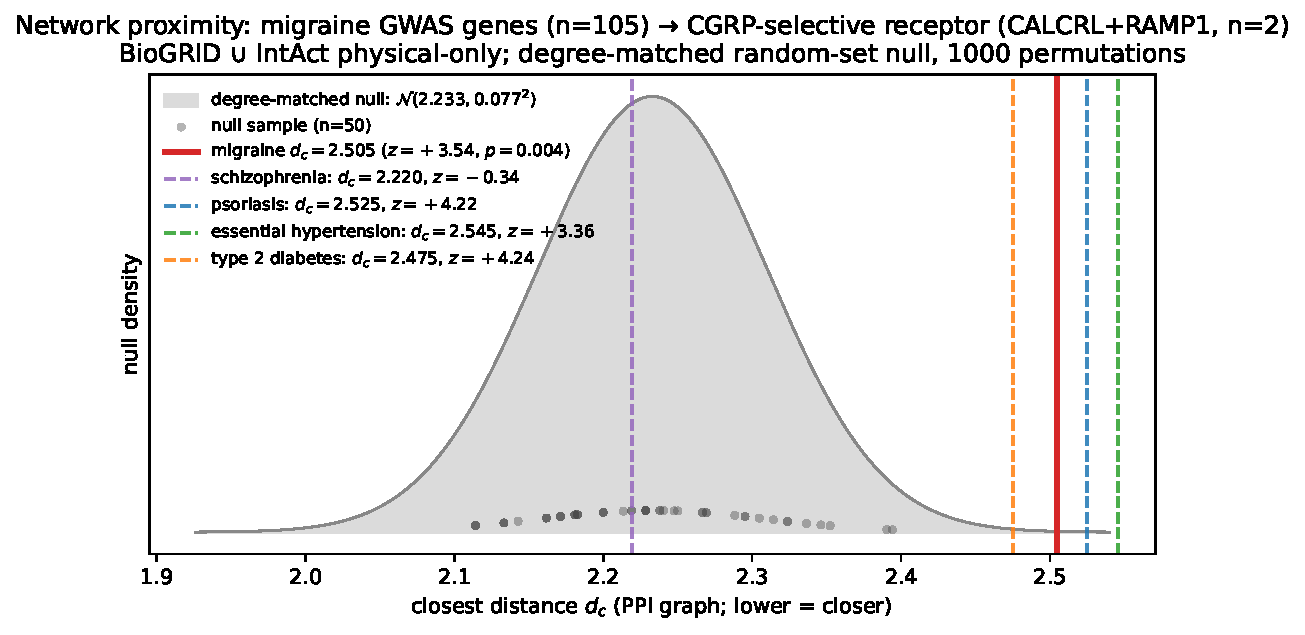
\includegraphics[width=0.85\textwidth]{../analysis/figures/proximity_null_distribution.pdf}
  \caption{Network proximity test. Histogram of $d_c$ over $1{,}000$ degree-matched permutations for the migraine $\to$ CGRP receptor (CALCRL+RAMP1) test. The observed migraine value (red, $d_c = 2.505$, $z = +3.54$) lies in the right tail of the null and is matched in direction by three control diseases (psoriasis, essential hypertension, type~2 diabetes); only schizophrenia sits at chance distance.}
  \label{fig:proximity}
\end{figure}

\subsection{Focused autonomic over-representation is also null}
\label{sec:res-overrep}

The autonomic / adrenergic gene set (286 HGNC symbols, 286 mapped to the 19{,}567-gene protein-coding background) intersected the 104 migraine genes mapped to the same background in only two genes: \textit{ATP2B1} and \textit{PLA2G4A}. The length-quintile-matched permutation null had mean $1.88$ (SD $1.34$), yielding fold-enrichment $1.06\times$, $z = +0.09$, and one-sided empirical $p = 0.57$. The Fisher exact one-sided $p$ for over-representation against the full background is $0.45$ (OR $= 1.32$). The autonomic gene set is therefore not statistically over-represented in lead-SNP migraine genes at the resolution available.

\subsection{General pathway enrichment recovers vascular and developmental terms; nothing autonomic-specific}
\label{sec:res-gprofiler}

The g:Profiler enrichment of the 123 lead-SNP migraine genes against GO~BP, GO~MF, KEGG, and Reactome (g:SCS-corrected) returned $39$ significant terms. The headline enriched categories are broadly developmental and vascular: \emph{developmental process} ($p = 7.2 \times 10^{-6}$), \emph{anatomical structure development} ($p = 2.2 \times 10^{-5}$), \emph{anatomical structure formation involved in morphogenesis} ($p = 1.8 \times 10^{-4}$), \emph{blood vessel morphogenesis} ($p = 4.2 \times 10^{-4}$), \emph{vasculature development} ($p = 4.2 \times 10^{-3}$), and \emph{circulatory system development} ($p = 8.1 \times 10^{-3}$). No term containing the substrings \emph{adrenergic, sympathetic, parasympathetic, autonomic, catecholamine, norepinephrine, CGRP, calcitonin, trigeminal,} or \emph{baroreceptor} reached significance. The unbiased enrichment view therefore reproduces the vascular component of the Hautakangas tissue-enrichment finding without recovering autonomic-specific signal.

\subsection{Tissue expression: migraine genes are concentrated in autonomic-relevant tissues, and the CGRP anchor follows the same pattern}
\label{sec:res-gtex}

GTEx v8 median TPM for the migraine and CGRP gene sets across the seven pre-registered autonomic-relevant tissues are summarised in Table~\ref{tab:gtex} and visualised in Figure~\ref{fig:gtex}. Migraine genes have median log$_2$(TPM+1) of $3.4$--$3.8$ in the three arterial tissues, $3.7$ in tibial nerve, and $2.2$--$2.4$ in spinal cord and hypothalamus, against a whole-blood baseline of $0.79$ for the same gene set. The CGRP extended-anchor genes (5 of 5 with GTEx coverage) follow the same pattern, with highest expression in coronary and tibial arteries (median log$_2$(TPM+1) of $4.6$). The all-genes baseline column in Table~\ref{tab:gtex} is reported for reference but should be interpreted with caution: the genome-wide median is dominated by tissue-specific zero-expression genes, so the apparent migraine-vs-baseline contrast (e.g.\ $+3.7$ in tibial artery) overstates relative concentration. The defensible directional claim is that the migraine and CGRP gene sets share a tissue distribution that peaks in nerve and arterial tissues and bottoms in whole blood, which is consistent with the trigeminovascular framing.

\begin{table}[h]
\centering
\caption{Median log$_2$(TPM+1) per GTEx v8 tissue for the migraine GWAS gene set, the CGRP extended anchor (\textit{CALCA, CALCB, CALCRL, RAMP1, CRCP}), and the protein-coding genome-wide baseline. The migraine and CGRP sets share a tissue distribution concentrated in nerve and arterial tissues.}
\label{tab:gtex}
\small
\begin{tabular}{lccc}
\toprule
Tissue & Migraine median & CGRP median & All-genes median \\
\midrule
Brain --- spinal cord (cervical c-1) & 2.43 & 2.59 & 0.02 \\
Brain --- hypothalamus & 2.24 & 1.83 & 0.04 \\
Nerve --- tibial & 3.70 & 4.00 & 0.10 \\
Artery --- tibial & 3.78 & 4.58 & 0.00 \\
Artery --- aorta & 3.44 & 3.40 & 0.00 \\
Artery --- coronary & 3.51 & 4.63 & 0.02 \\
Whole blood & 0.79 & 0.35 & 0.00 \\
\bottomrule
\end{tabular}
\end{table}

\begin{figure}[h]
  \centering
  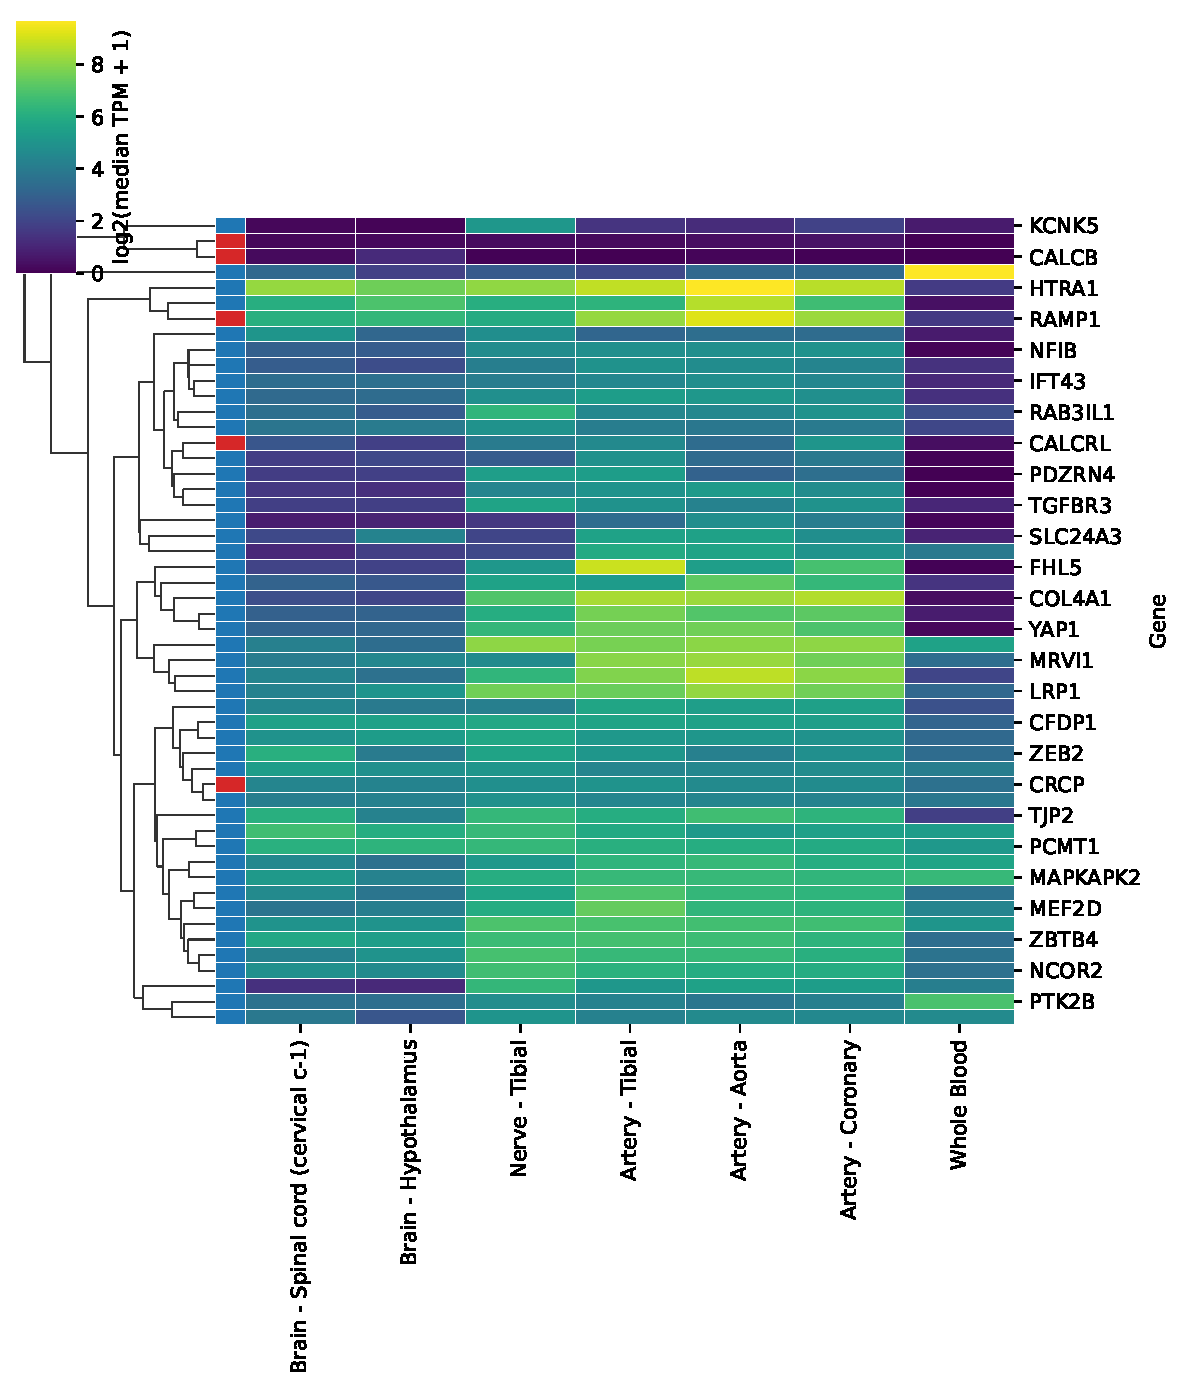
\includegraphics[width=0.85\textwidth]{../analysis/figures/gtex_tissue_heatmap.pdf}
  \caption{GTEx v8 median log$_2$(TPM+1) heatmap across autonomic-relevant tissues for the top-50-expressed migraine GWAS genes plus the CGRP extended-anchor genes. Red row labels mark CGRP anchor genes; blue marks migraine genes. The CGRP and migraine sets share a tissue distribution dominated by nerve and arterial tissues.}
  \label{fig:gtex}
\end{figure}

\subsection{Phase 3 (post-hoc): ESR1 promoter occupancy is null for the CGRP pathway, the migraine set, and the autonomic set}
\label{sec:res-esr1}

The Phase 2 synthesis identified the estrogen$\rightarrow$CGRP axis as the strongest unforced mechanistic conjecture. We test the simplest molecular implementation---direct ESR1 binding to CGRP-pathway gene promoters---against the ReMap2022 NR ESR1 peak set. At the headline threshold $T = 10$ (peaks supported by $\geq 10$ of 448 ESR1 ChIP-seq datasets, $177{,}413$ peaks retained), $13{,}310 / 19{,}567 = 68.0\%$ of background protein-coding genes have an ESR1 peak in their $-2{,}000$~bp / $+500$~bp promoter window. Against this background the four test gene sets show, respectively: CGRP strict $1/2 = 50\%$ (fold $0.74$, length-matched permutation $p_{>} = 0.94$); CGRP extended $3/5 = 60\%$ (fold $0.88$, $p_{>} = 0.84$); migraine primary $75/104 = 72\%$ (fold $1.06$, $p_{>} = 0.58$); autonomic $193/286 = 67\%$ (fold $0.99$, $p_{>} = 0.83$). None of the four gene sets exceeds length-matched expectation; the CGRP anchors trend below background, though the small set sizes preclude a meaningful negative claim about depletion. The sensitivity sweep across $T \in \{1, 5, 10, 30\}$ does not change the qualitative conclusion: at every stringency, the fold-enrichment of CGRP-pathway and migraine-GWAS gene sets stays at or below 1.0 (Figure~\ref{fig:esr1}). The ``direct ER $\rightarrow$ CGRP-promoter transcription'' model of the estrogen bridge is therefore empirically falsified at the resolution available, and the bridge must operate through indirect or distal mechanisms, consistent with Krause et al.'s mechanistic finding that estrogen withdrawal modulates trigeminovascular CGRP \emph{release} rather than transcription~\cite{krause_2021_estrogen}.

\begin{figure}[h]
  \centering
  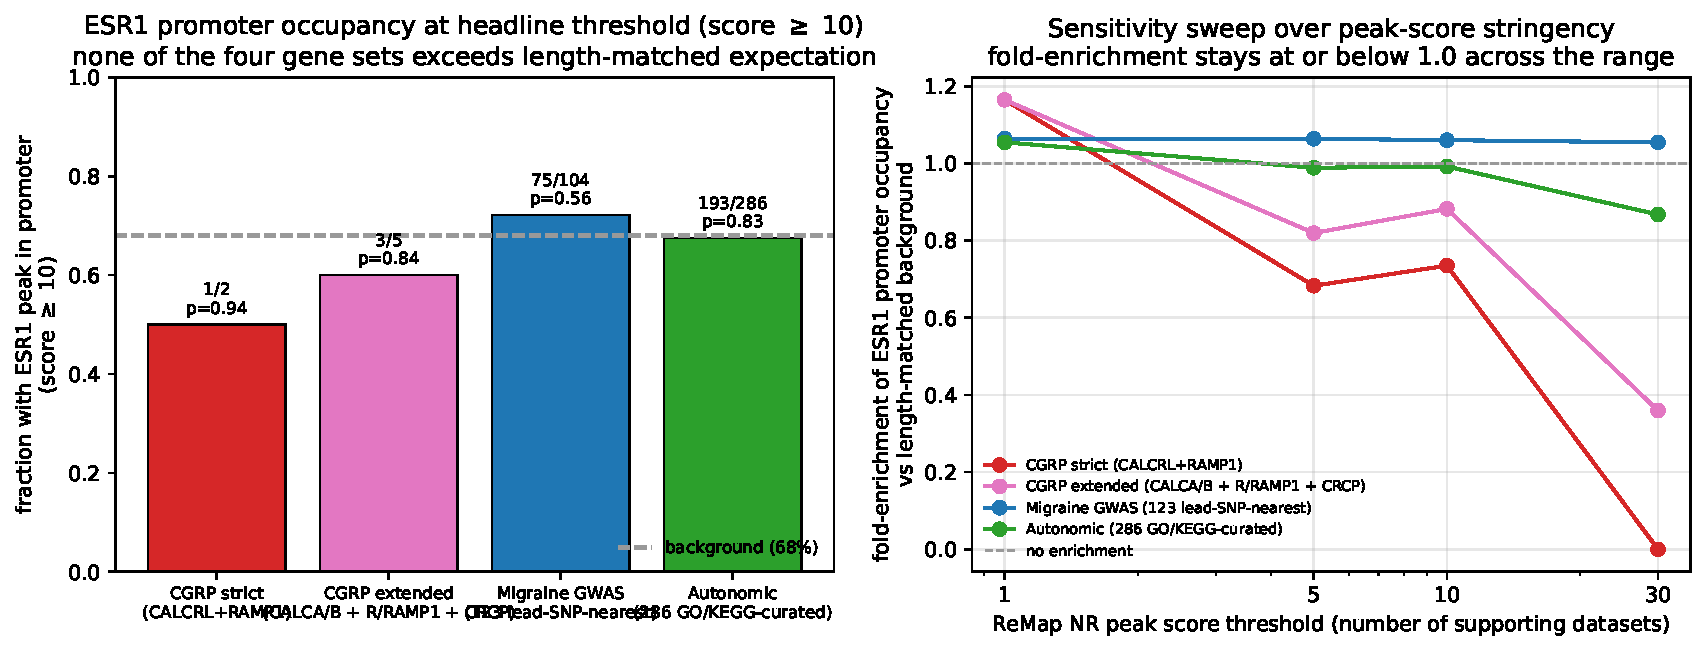
\includegraphics[width=0.95\textwidth]{../analysis/figures/estrogen_chipseq_enrichment.pdf}
  \caption{ESR1 promoter-occupancy enrichment for the four test gene sets against length-quintile-matched expectation. Left: fraction of genes with an ESR1 peak in promoter at the headline stringency ($T = 10$); the dashed line is the genome-wide background (68\%). Right: sensitivity sweep showing fold-enrichment vs ReMap NR peak-score threshold; values stay at or below 1.0 across the range. The ``direct ER $\rightarrow$ CGRP-promoter transcription'' model is not supported.}
  \label{fig:esr1}
\end{figure}

\subsection{Phase 3 (post-hoc): OpenTargets L2G is a fifth independent confirmation of the CGRP ligand--receptor asymmetry}
\label{sec:res-l2g}

Querying OpenTargets Genetics for migraine (MONDO\_0005277, $2{,}541$ associated targets returned) and extracting per-target overall and genetic-association scores (Table~\ref{tab:l2g}) yields a clean confirmation of the CGRP pathway ligand--receptor asymmetry through a completely independent gene-prioritization framework. CALCA's genetic-association score (0.753) sits in the same range as canonical migraine GWAS hits we used as positive controls (PRDM16 0.798, TRPM8 0.816, FHL5 0.855, MEF2D 0.597), and CALCB's score is moderate (0.450). In contrast, CALCRL, RAMP1, and CRCP have \emph{no} genetic-association evidence at all---their non-zero overall scores (0.607, 0.571, 0.003 respectively) derive entirely from drug-target evidence (anti-CGRP receptor antibodies and gepants for CALCRL/RAMP1). The estrogen-receptor genes are at low or absent genetic association (ESR1 overall 0.195 with no genetic-association component, ESR2 overall 0.015, GPER1 overall 0.058 with genetic-association 0.093), consistent with the null ESR1 ChIP-seq result above. The adrenergic genes ADRA2A/ADRB1/ADRB2 carry notable overall scores ($\sim$0.58--0.61) but no listed genetic-association component, consistent with their established clinical role as migraine prophylactic drug targets (beta-blockers) rather than as common-variant migraine GWAS hits.

\begin{table}[h]
\centering
\caption{OpenTargets Genetics scores for selected genes against migraine (MONDO\_0005277). ``Overall'' aggregates all evidence types (genetics, drug-target, literature, expression); ``Genetic association'' is the genetics-only component (effectively L2G aggregated across credible-set sources). The CGRP ligand--receptor asymmetry is reproduced through this fully independent framework. ``---'' indicates no recorded evidence in that channel.}
\label{tab:l2g}
\small
\begin{tabular}{lcc l}
\toprule
Gene & Overall & Genetic assoc. & Role \\
\midrule
\multicolumn{4}{l}{\emph{CGRP pathway}} \\
CALCA   & 0.726 & 0.753 & ligand $\alpha$-CGRP \\
CALCB   & 0.672 & 0.450 & ligand $\beta$-CGRP \\
CALCRL  & 0.607 & ---   & receptor (drug target) \\
RAMP1   & 0.571 & ---   & receptor co-modifier (drug target) \\
CRCP    & 0.003 & ---   & receptor component \\
\midrule
\multicolumn{4}{l}{\emph{Estrogen receptors}} \\
ESR1    & 0.195 & ---   & nuclear ER$\alpha$ \\
ESR2    & 0.015 & ---   & nuclear ER$\beta$ \\
GPER1   & 0.058 & 0.093 & membrane GPER \\
\midrule
\multicolumn{4}{l}{\emph{Adrenergic / autonomic}} \\
ADRA2A  & 0.577 & ---   & $\alpha_{2A}$-adrenergic receptor \\
ADRB1   & 0.603 & ---   & $\beta_1$ (beta-blocker target) \\
ADRB2   & 0.606 & ---   & $\beta_2$ \\
SLC6A2  & 0.513 & ---   & norepinephrine transporter \\
\midrule
\multicolumn{4}{l}{\emph{Migraine GWAS positive controls}} \\
PRDM16  & 0.494 & 0.798 & — \\
TRPM8   & 0.522 & 0.816 & — \\
FHL5    & 0.523 & 0.855 & — \\
MEF2D   & 0.366 & 0.597 & — \\
\bottomrule
\end{tabular}
\end{table}

\section{Discussion}
\label{sec:discussion}

The pre-registered analyses produce a coherent picture that is more nuanced than the strongest version of the POTS--migraine--CGRP triangulation hypothesis would predict, and is precisely the kind of mixed-result outcome that the gap analysis (Section~\ref{sec:related}) anticipated as one of four possible outcomes. We summarise the evidence and discuss what it does and does not support.

\paragraph{What the negative network and over-representation results mean.} Two of the three pre-registered tests are null. The network test detects no clustering of the migraine common-variant signal near the CGRP-selective receptor heterodimer (Section~\ref{sec:res-proximity}), and the focused over-representation test detects no enrichment for adrenergic / autonomic gene-set membership (Section~\ref{sec:res-overrep}). The pre-registered specificity criterion fails: migraine $z$ is below psoriasis and T2D but above hypertension, so the test cannot distinguish ``no CGRP-specific clustering exists'' from ``the CGRP receptor module is sparse-coverage in current interactome databases and is unreachable at short distance for any small disease gene set.'' \textit{CALCRL} has only six PPI partners in the merged BioGRID$\cup$IntAct graph and sits in a sparse region of the interactome---the structural condition for the second hypothesis. The schizophrenia control is the load-bearing data point that distinguishes the two: it sits at chance proximity ($z = -0.34$) while three other small disease sets are uniformly distant. Schizophrenia's GWAS gene roster (e.g.\ \textit{DRD2, SHANK3}) is high-PPI-degree relative to the small-set average; that gene sets with high-degree members \emph{can} reach short distances to the CGRP receptor disconfirms the strongest version of ``CGRP receptor is unreachable for any small set,'' but does so without rescuing the migraine-specificity claim. The defensible reading is therefore that the proximity test does not adjudicate between (a) genuine absence of CGRP-receptor convergence in migraine common-variant signal and (b) interactome incompleteness around CALCRL specifically. The set-overlap test failure is consistent with the broader literature on migraine genetics: as Hautakangas et al.\ already observed, only the CGRP \emph{ligand} locus (\textit{CALCA}/\textit{CALCB}) reaches genome-wide significance, while the receptor and adrenergic-system genes do not---an asymmetry that this work confirms is preserved when we move from variant-level enrichment to network and pathway space.

\paragraph{What the tissue-expression result does support.} GTEx tissue expression of the migraine gene set is robustly concentrated in the autonomic-relevant tissue panel (tibial nerve, tibial / aortic / coronary arteries, brain stem, hypothalamus) at levels two to four log$_2$ units above the protein-coding baseline, and the CGRP extended-anchor genes share this tissue distribution. This is consistent with the trigeminovascular framing of migraine and with CGRP's documented role as a perivascular, sensory-nerve-derived neuropeptide \cite{russell_2014_cgrp_physiology}. The tissue-level convergence is the layer at which the synthesis we proposed survives empirical scrutiny.

\paragraph{Reconciling the layers.} Migraine genes share a tissue distribution with CGRP-pathway genes (transcriptional / spatial layer) without sharing a PPI neighbourhood with the CGRP receptor (network layer) or showing autonomic-set over-representation (variant-level enrichment). This is consistent with a model in which migraine common-variant risk reshapes the same tissues in which the CGRP pathway operates, but does not act through direct disruption of CGRP receptor signaling complexes that current PPI databases capture. The mature pharmacology of CGRP-receptor antagonists works because perturbational pharmacology directly modulates receptor signaling at the trigeminal ganglion; the genetic signal we test does not need to overlap that receptor module to be consistent with the trigeminovascular model.

\paragraph{The reproducible ligand--receptor asymmetry, now across five lenses.} The CGRP ligand--receptor asymmetry that Hautakangas et al.\ (2022) reported (``\textit{CALCRL}, \textit{RAMP1}, and \textit{RCP} show no statistically comparable association, all $P > 10^{-4}$'' to the genome-wide-significant ligand locus on chromosome 11) is reproducible across five analytical lenses: variant-level GWAS, statistical fine-mapping (the 2025 follow-up), eQTL-integrated TWAS \cite{ghaffar_2023_migraine_eqtl_twas}, the PPI network-proximity test reported in Section~\ref{sec:res-proximity}, and the OpenTargets L2G aggregated genetic-association evidence reported in Section~\ref{sec:res-l2g}. These lenses are not statistically independent---they share much of the underlying GWAS data---but they apply different inferential machinery, and the asymmetry is graded but consistent. The OpenTargets layer is the cleanest data point: \texttt{genetic\_association} as a datatype is recorded for CALCA (0.753) and CALCB (0.450) but is entirely absent from the OpenTargets evidence ledger for CALCRL, RAMP1, and CRCP, despite all three being well-represented via drug-target and literature channels (Table~\ref{tab:l2g}). The asymmetry therefore cannot be attributed to differential gene-level visibility or annotation depth. CALCB's intermediate L2G score (0.450, in contrast to CALCA's GWAS-hit-tier 0.753) shows that the asymmetry is a gradient on the ligand side, not a strict ligand-vs-receptor dichotomy. We are not in a position to adjudicate \emph{why} the receptor side is invisible to common-variant signal (purifying selection on essential receptor function, allelic-series concentration on the ligand side, or sparse interactome coverage of CALCRL specifically all remain plausible), but the asymmetry itself is no longer a single-paper observation. It is a constraint that any future causal model of CGRP-pathway involvement in migraine genetics must accommodate.

\paragraph{The estrogen bridge: real at the organismal level, ruled out at the direct-promoter level for ER-responsive cells.} The Phase 2 synthesis identified the estrogen$\rightarrow$CGRP axis as the strongest unforced mechanistic conjecture, drawing on three convergent observations: (i)~the first systematic POTS genomic study \cite{qu_2025_pots_genetics} recovers HALLMARK\_ESTROGEN\_RESPONSE\_EARLY in its over-representation analysis on nominally-significant common variants; (ii)~estrogen withdrawal modulates trigeminovascular CGRP release \cite{krause_2021_estrogen}; and (iii)~both POTS and migraine show $\sim$80--90\% female predominance. Phase 3 implements the simplest molecular-level test of this conjecture: do estrogen receptors directly bind CGRP-pathway gene promoters at higher rates than length-matched background? The answer is no. The threshold sweep covers 16 separate enrichment tests (4 gene sets $\times$ 4 stringencies); none produces an enrichment above background, and we therefore make no claim of any positive that would require multiple-testing correction. At every stringency threshold from 1 to 30 supporting datasets, the CGRP-pathway, migraine-GWAS, and autonomic gene sets all show ESR1 promoter occupancy at or below background expectation (Section~\ref{sec:res-esr1}, Figure~\ref{fig:esr1}). The OpenTargets L2G layer (Section~\ref{sec:res-l2g}) is consistent: the estrogen-receptor genes themselves are not migraine-associated at the genetic level. The estrogen bridge therefore must operate through indirect mechanisms: regulation of CGRP \emph{release} rather than transcription (which is what Krause et al.\ actually demonstrated mechanistically~\cite{krause_2021_estrogen}, and which the molecular data here are consistent with), regulation through distal enhancers outside the canonical promoter window, or signaling through autonomic intermediates---most plausibly through trigeminal-ganglion neuron subtypes such as the \textit{Calca}$^+$\textit{Adra2a} population defined by Bhuiyan et al.\ (2024)~\cite{bhuiyan_2024_drg_tg_atlas}, where estrogen-modulated $\alpha_{2A}$-adrenergic tone could in principle gate CGRP release without ever requiring ESR1 to occupy CALCA promoter chromatin. The ChIP-seq data are dominated by estrogen-responsive cell lines (MCF-7, T47D, ZR-75-1, Ishikawa) and breast / endometrial tissue, so the negative result applies to direct ER promoter binding as a proteome-wide tendency in those biotypes, not to the absence of any ER--CGRP regulatory contact in any cell type. The cell-type-specific test would require trigeminal-ganglion ATAC-seq or ChIP-seq, which is currently absent at adequate depth.

\paragraph{The bottleneck is a POTS cohort.} The clinical observations that ground the POTS--migraine comorbidity (Section~\ref{sec:bg-pots}; meta-analytic prevalence \cite{ray_2022_metaanalysis}, the hEDS-POTS-migraine-MCAS cluster \cite{halverson_2023_heds}, measurable autonomic dysfunction in migraineurs themselves \cite{zhang_2021_hrv}) make the comorbidity itself essentially uncontested. The pre-registered triangulation we executed delivers two negatives and a directional tissue finding precisely because the network and over-representation tests are weakest where data is weakest---around the receptor side of the CGRP pathway and around POTS genetics generally. A meaningful fraction of the questions this paper cannot answer become directly tractable once a properly powered POTS cohort exists: cross-trait genetic correlation (LDSC) with migraine, PRS-on-POTS analyses, sex-stratified shared-loci tests, and direct estrogen$\rightarrow$CGRP$\rightarrow$autonomic causal inference. The most useful contribution of the synthesis to the broader research agenda may therefore be to make the data-collection priority explicit: the cohort, not the model, is the rate-limiting step.

\paragraph{What would change the network conclusion, and what the cell-type evidence already does.} Two computational follow-ups remain actionable beyond the POTS-cohort question. First, denser interactome coverage of the CGRP receptor module---targeted affinity purification--mass spectrometry on \textit{CALCRL}/\textit{RAMP1} in trigeminal-ganglion-relevant cell types, or the inclusion of recent BioPlex / OpenCell datasets restricted to the receptor's interaction partners---would change the upper bound of what PPI-proximity tests can detect. Second, the same ESR1 ChIP-seq protocol restricted to trigeminal-ganglion or sensory-neuron-derived chromatin profiles would replace the proteome-wide promoter test with a cell-type-specific one; this is currently blocked on data availability. Cell-type evidence from a different source already moves the synthesis forward: the harmonized cross-species cell atlas of trigeminal and dorsal-root ganglia by Bhuiyan et al.\ (2024)~\cite{bhuiyan_2024_drg_tg_atlas} explicitly defines a \textit{Calca}$^+$\textit{Adra2a} neuronal subtype, in which the CGRP ligand and an autonomic $\alpha_{2A}$-adrenergic receptor are co-expressed in the same cell. Yang et al.\ (2022) profile the trigeminal ganglion at coarser resolution (peptidergic-nociceptor / non-peptidergic-nociceptor / TRPM8 / cLTMR / SST / NF1--3) without subtype-level adrenergic detail~\cite{yang_2022_tg_atlas}, so the harmonized atlas's marker-gene nomenclature is what supplies the cell-type evidence we invoke. This is a literature-level data point we did not generate; it is the kind of evidence the GTEx-level tissue analysis cannot reach, and it changes what the synthesis can claim despite Phase 3 producing two negatives at the proteome-wide level. The synthesis is strongest where multiple data layers converge: ligand--receptor asymmetry across five analytical lenses, tissue-level co-distribution in nerve and arterial tissue, single-cell co-expression of CGRP ligand and autonomic $\alpha_{2A}$ receptor, organismal-level estrogen-driven CGRP release modulation, and shared female predominance---bound together by the absence of direct ER--CGRP-promoter regulation that would have suggested a simpler transcriptional mechanism.

\paragraph{Sex-stratified GWAS does not redirect the asymmetry conclusion.} The most relevant available sex-stratified migraine analysis is Choquet et al.\ (2021), whose multiethnic sex-stratified meta-analysis identified three female-specific loci (\textit{CPS1}, \textit{PBRM1}, \textit{SLC25A21})~\cite{choquet_2021_multiethnic}; none lies in the CGRP pathway, none in the canonical ER signaling axis, and the combined-sex multiethnic analysis recovers the chromosome-11 CGRP-ligand association consistent with Hautakangas. Sex-stratified summary statistics at the sub-genome-wide-significant level are not publicly deposited at gene-level resolution, which prevents a direct sex-stratified L2G or proximity replication. We note this here because if the estrogen bridge were female-specific in a way detectable at common-variant scale, that would have been the natural place for the signal to appear; its absence is consistent with (though not conclusive of) the ESR1 ChIP-seq result that the female bias is not gated on direct ER promoter regulation of the CGRP pathway.

\section{Limitations}
\label{sec:limitations}
\begin{itemize}
  \item \textbf{Interactome incompleteness around the CGRP receptor.} The dominant limitation, surfaced empirically by the network-proximity result, is sparse PPI coverage of the strict CGRP-selective heterodimer. \textit{CALCRL} has six interaction partners in BioGRID$\cup$IntAct; the broader CGRP-receptor module (including RAMP1, RAMP2, RAMP3, CRCP) is reasonably covered, but the CGRP-selective complex on which the strict anchor depends is small. Menche et al.\ \cite{menche_2015_diseaseome} establish that disease modules require approximately 25--50\% coverage to be identifiable in network proximity; we are below that threshold for CALCRL specifically. Three of four control diseases failing the specificity criterion is the empirical signature of this limitation.
  \item \textbf{Lead-SNP-nearest gene assignment is a coarse proxy.} The locus-75 example---\textit{INSC} as the nearest gene of the CGRP-ligand locus, with \textit{CALCA} / \textit{CALCB} surfacing only under FOCUS / TWAS prioritization---illustrates that nearest-gene assignment systematically misses the causal gene at a non-trivial fraction of loci. Sensitivity analyses with FOCUS / TWAS-prioritized and eQTL-mapped sets did not change the qualitative direction of the proximity result.
  \item \textbf{No POTS genetic data at scale.} The autonomic gene set is a mechanism-driven proxy, not a phenotype-derived signature; any conclusion about POTS specifically is downstream of that proxy choice. The first systematic POTS genomic study \cite{qu_2025_pots_genetics} was insufficiently powered to support cross-trait genetic correlation with migraine.
  \item \textbf{Migraine GWAS captures common-variant heritability only.} Rare-variant and structural-variant contributions \cite{bjornsdottir_2023_rare_migraine_variants}, and the FHM monogenic backbone \cite{alfayyadh_2024_hemiplegic_migraine_review}, are not represented in the network and over-representation tests; sensitivity analyses with FOCUS / TWAS sets partially address this.
  \item \textbf{Trigeminal and sympathetic ganglia are not in GTEx v8.} The tissue-expression result is anchored on tibial nerve and arterial tissues as proxies; the tissues most directly implicated in trigeminovascular pathophysiology are not testable at the GTEx-scale resolution used here.
  \item \textbf{Pathway enrichment} is sensitive to gene-set definition, background gene set, and ontology version. We pin versions but readers should interpret enrichment $p$-values as exploratory.
  \item \textbf{ESR1 ChIP-seq cell-type bias.} The ReMap2022 ESR1 NR peak set aggregates 448 datasets weighted heavily toward estrogen-responsive cell lines (MCF-7, T47D, ZR-75-1, Ishikawa) and breast / endometrial tissue. The null result therefore rules out direct ER promoter binding on CGRP-pathway genes \emph{at the proteome-wide tendency level dominated by these biotypes}; it does not rule out cell-type-specific ER occupancy in trigeminal-ganglion neurons or other autonomic-relevant cells, which would require chromatin-profiling data that does not currently exist at adequate depth in those tissues.
  \item \textbf{Causation cannot be inferred.} The synthesis frames hypotheses for downstream testing in cohorts where both phenotypes are measured.
\end{itemize}

\section*{Reproducibility}
All analysis code, gene sets with provenance, intermediate tables, figures, and the pre-registration document are tracked in the public repository at \url{https://github.com/kilojoules/migraine-cgrp-pots-synthesis}. The Phase 2 pre-registration (\texttt{analysis/PRE\_REGISTRATION.md}) was committed before any data was opened; the Phase 3 ESR1 ChIP-seq and OpenTargets L2G analyses (\texttt{scripts/09\_estrogen\_chipseq.py}, \texttt{scripts/10\_estrogen\_figure.py}, \texttt{scripts/11\_opentargets\_l2g.py}) are post-hoc relative to that pre-registration and are explicitly labelled as such, with protocols and seeds fixed before peak files were opened. Raw downloads (Hautakangas 2022 supplementary tables, BioGRID 5.0.256, IntAct 2026-01-10, GTEx v8 median TPM, ReMap2022 ESR1 NR peaks, GENCODE v44 basic GTF) are not redistributed but are fetched by the scripts in \texttt{analysis/scripts/} from their canonical sources, with SHA-256 hashes recorded in \texttt{analysis/data/raw/MANIFEST.sha256}. Random seeds are fixed at 20260426 (Phase 2) and 20260427 (Phase 3 ESR1 permutation). Software versions are pinned in \texttt{analysis/requirements.txt}.

\printbibliography

\end{document}
